% Chapter Template

\chapter{Experiments evaluation} % Main chapter title

\label{Chapter5} % Change X to a consecutive number; for referencing this chapter elsewhere, use \ref{ChapterX}
In this section we present the results of our experiments in detail. In the first two sections we compare the estimated positions of the three tested algorithms at the given checkpoints. Firstly the results of experiments with wide spread anchors are indicated, secondly the results with nearer anchor positions are shown. In a third section we justify the differences between these two scenarios and comment the accuracy of the results. In the last section we conclude our work and propose next improvement steps for our algorithm. 

%----------------------------------------------------------------------------------------
%	SECTION 1
%----------------------------------------------------------------------------------------

\section{Indoor positioning results with low density of anchor nodes}
In the following the results of our algorithms with a wide distance between anchor nodes are shown. Within this setup we tested trajectory 1 to 4. Each trajectory was tested five times, the results are shown as arithmetic means of these five probes. The anchor node positions for these four tested trajectories are indicated in figure \ref{fig:anchor_position}.

In the first trajectory, the arithmetic mean (hereafter often called average) distance error over all checkpoints was 1.53 meter for $PF_{full}$, 1.47 meter for $PF_{UWBonly}$ and 1.69 meter for Sequiturs commercial system. Looking at figure \ref{fig:trajectory1and2_results}, we see that the errors are often smaller than 1.5 meter, however, there are some checkpoints with very low accuracy. This is also emphasized by comparing the arithmetic mean error to the median error of 1.22m for $PF_{full}$, 0.68m for $PF_{UWBonly}$ and 1.14m for Sequitur, which are significantly lower than the arithmetic means.

The measurements for trajectory two were almost identical, except for $PF_{UWBonly}$, which had no outliers during trajectory 2. The arithmetic mean error for $PF_{full}$ was 2.36m, for $PF_{UWBonly}$ it was 0.55m and for Sequitur 2.26m. Except for $PF_{UWBonly}$, the median errors were again a lot more accurate with 1.07m for $PF_{full}$, 0.49m for $PF_{UWBonly}$ and 1.73m for Sequitur.

\begin{figure}[th]
\centering
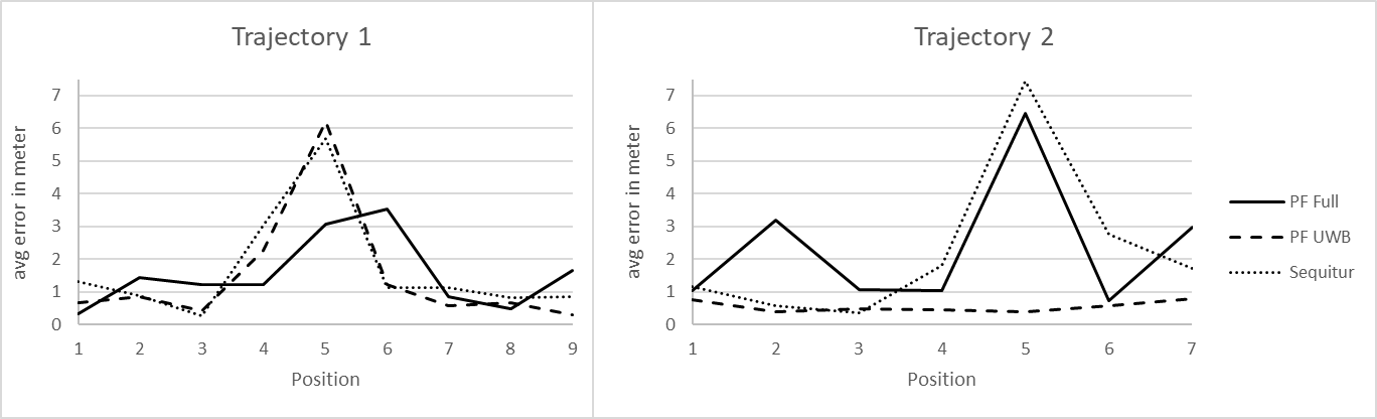
\includegraphics[width=1.0\textwidth]{Figures/trajectory1_2_results}
\decoRule
\caption[Positioning results trajectory 1 and 2]{Graphs of measured distance errors at each checkpoint in trajectory 1, respectively trajectory 2.}
\label{fig:trajectory1and2_results}
\end{figure}

The results for trajectory 3 and 4 were rather similar, however, the peaks observed in figure \ref{fig:trajectory3and4_results} were not as extreme as for the first two trajectories. As above, the average errors in the third trajectory of 1.18m for $PF_{full}$, 0.80m for $PF_{UWBonly}$ and 1.87m for Sequitur were also mentionable higher than the medians of 0.92m, 0.76m and 1.60m.

In the last of these four trajectories no big outliers were stated. Nonetheless the average errors of 1.72m, 1.51m and 1.52m, as well as the median errors 1.26m, 0.68m and 1.24m for $PF_{full}$, $PF_{UWBonly}$ and Sequitur, were still not as accurate as intended.

\begin{figure}[th]
\centering
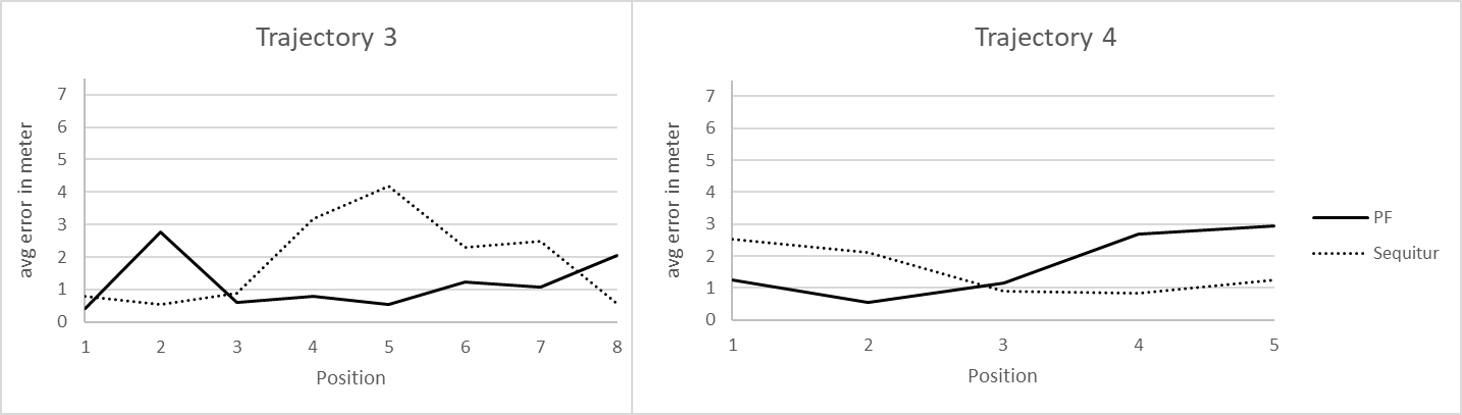
\includegraphics[width=1.0\textwidth]{Figures/trajectory3_4_results}
\decoRule
\caption[Positioning results trajectory 3 and 4]{Graphs of measured distance errors at each checkpoint in trajectory 3, respectively trajectory 4.}
\label{fig:trajectory3and4_results}
\end{figure}

Having a closer look at table \ref{tab:arithmetic_errors}, we see that surprisingly the version of the particle filter only using UWB was the best on every of the trajectories in the low-density anchor node test environment. Moreover, we have seen that there are very big differences between the single checkpoints and even between trajectories. The full variant of the particle filter and the Sequitur system have similar accuracies. For some trajectories one of the algorithms is better, for other trajectories the other performs better. Possible reasons for these volatile results are discussed in the upcoming section \ref{Section2}. 

\begin{table}
\caption{The arithmetic mean of errors in trajectory 1 to 4 and in total over all measured checkpoints for the three algorithms.}
\label{tab:arithmetic_errors}
\centering
\begin{tabular}{l l l l}
\toprule
\textbf{Trajectory} & \textbf{PF Full} & \textbf{PF UWB} & \textbf{Sequitur}\\
\midrule
\textbf{T1} & 1.54 & 1.47 & 1.69\\
\textbf{T2} & 2.36 & 0.55 & 2.26\\
\textbf{T3} & 1.18 & 0.80 & 1.87\\
\textbf{T4} & 1.72 & 1.51 & 1.52\\
\midrule
\textbf{total}  & \textbf{1.61} & \textbf{1.03} & \textbf{1.79}\\
\bottomrule\\
\end{tabular}
\end{table}

%----------------------------------------------------------------------------------------
%	SECTION 2
%----------------------------------------------------------------------------------------

\section{Comments on low density anchor node test results}
\label{Section2}
The test results in the experiment setup with wide anchor node distances were not as good as intended. To find the reasons for that, we have to carefully have a look at the underlying implementation and the single checkpoint circumstances. We identified two main causes for bad results, they are explained in detail during the next two subsections.
\begin{itemize}
\item Checkpoints outside of AN bounding boxes
\item Failing UWB connection due to too wide distances to ANs
\end{itemize}

\subsection{Bounding box restrictions}
The AN positions naturally form a bounding box around the environment. The bounding box is the area spanned by straight connections between anchor nodes, as indicated in figure \ref{fig:trajectory1_boundingBox}. Trilateration, also with small distance errors, works well within the bounding box. However even small ranging errors can lead to wrong position estimations outside the bounding box. 
\begin{figure}[th]
\centering
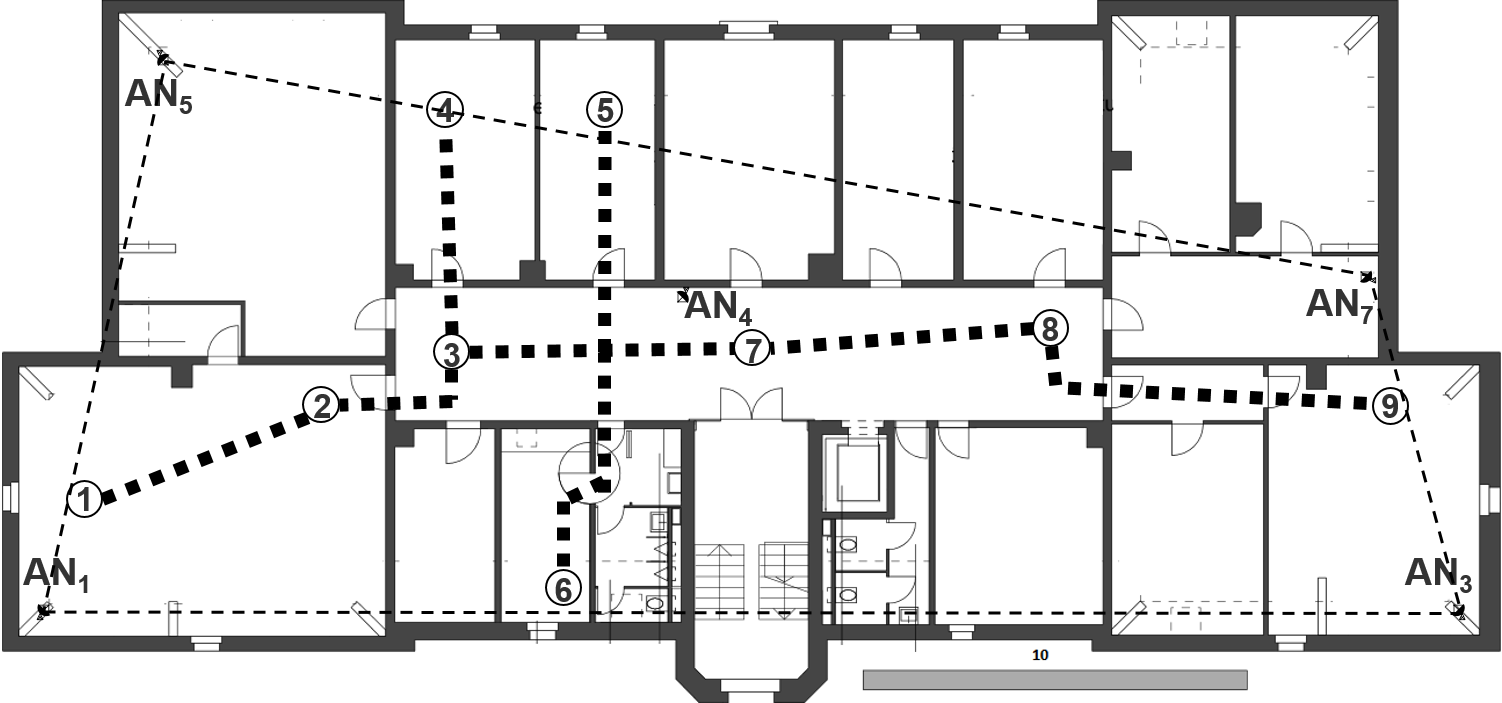
\includegraphics[width=0.8\textwidth]{Figures/trajectory1_boundingBox}
\decoRule
\caption[Bounding box and checkpoints for trajectory 1 ]{Indicated bounding box of the anchor node positions for trajectory 1.}
\label{fig:trajectory1_boundingBox}
\end{figure}
In our experiment especially the results on checkpoint 5 in trajectory 1 and 2 stand out. The average measured errors of 3.09m for $PF_{full}$, 6.23m for ${PF_UWBonly}$ and 5.70m for Sequitur during the first trajectory and 6.46m,  0.38m and 7.45m during the second trajectory are way higher than for other checkpoints. The fact that all of the three algorithms had troubles estimating this position, leads to the conclusion that the experiment setup was the main reason for the big errors at this checkpoint. Moreover, not only lies this point outside the bounding box, but it was also far away from the nearest ANs without line of sight.

\subsection{Failing UWB connections}
All three algorithms depend on a good established UWB connection, as all the ANs ranging estimations are only transmitted via UWB. Especially in the full implementation of the particle filter many UWB meassages are transmitted, because fingerprinting and IMU data are additionally exchanged. For this purpose the radio mode of the UWB devices had to be set to 2, which led to a higher datarate with the cost of lower possible communication distances.
For certain checkpoints the distance to the farest anchor nodes were even more than 35m, which was too much for a stable UWB connection with the mentioned configuration. Particularly the full particle filter had troubles receiving enough usable data, as it produced more overhead than the other algorithms. This led to a high package loss for the full version, such that only one or two range measurements per estimation step were taken into account - instead of the possible five - leading to a higher error. 


%----------------------------------------------------------------------------------------
%	SECTION 3
%----------------------------------------------------------------------------------------

\section{Indoor positioning results with high density of anchor nodes}
By 

%-----------------------------------
%	SUBSECTION 1
%-----------------------------------
\subsection{Transmission}
Here goes the text.
%-----------------------------------
%	SUBSECTION 2
%-----------------------------------
\subsection{Ranging with TWR}
Here goes the text.

%----------------------------------------------------------------------------------------
%	SECTION 4
%----------------------------------------------------------------------------------------

\section{Comments on high density anchor node test results}
\label{Section4}
Here goes the text.
\begin{itemize}
\item Spread the particles and validate new positions with floormap constraints
\item Evaluate UWB ranges, IMU measures and zone indication to assign likelihood
\item Calculate weight function and systematically resample (and reposition) particles with low weights
\item Sum up weighted positions
\end{itemize}

%-----------------------------------
%	SUBSECTION 1
%-----------------------------------
\subsection{Inputs}
Here goes the text.



%-----------------------------------
%	SUBSECTION 2
%-----------------------------------
\subsection{Likelihood and weighting}
Here goes the text.


%-----------------------------------
%	SUBSECTION 3
%-----------------------------------
\subsection{Ranging with TWR}
Here goes the text.



%----------------------------------------------------------------------------------------
%	SECTION 4
%----------------------------------------------------------------------------------------

\section{Conclusion and further work}
Here goes the text.
\begin{itemize}
\item Spread the particles and validate new positions with floormap constraints
\item Evaluate UWB ranges, IMU measures and zone indication to assign likelihood
\item Calculate weight function and systematically resample (and reposition) particles with low weights
\item Sum up weighted positions
\end{itemize}
